\begin{filecontents*}{referencias.bib}
@dataset{uci_ctg,
  author       = {{UCI Machine Learning Repository}},
  title        = {Cardiotocography},
  date         = {2010},
  publisher    = {University of California, Irvine},
  doi          = {10.24432/C51S4N},
  url          = {https://doi.org/10.24432/C51S4N}
}

@article{ayres2000sisporto,
  author       = {Ayres-de-Campos, Diogo and Bernardes, Jo{\~{a}}o and Costa-Pereira, Ant{\'o}nio and Pereira-Leite, Lu{\'i}s},
  title        = {SisPorto 2.0: A program for automated analysis of cardiotocograms},
  journaltitle = {Journal of Maternal-Fetal Medicine},
  year         = {2000},
  volume       = {9},
  number       = {5},
  pages        = {311--318},
  doi          = {10.1002/1520-6661(200009/10)9:5<311::aid-mfm12>3.0.co;2-9}
}

@online{zucco_ml,
  author       = {Ju\'arez Zucco, Leonardo},
  title        = {Machine Learning desde Cero},
  organization = {JetBrains Marketplace},
  url          = {https://plugins.jetbrains.com/plugin/35104-machine-learning-desde-cero/versions#tabs},
  urldate      = {2026-11-14},
  note         = {Recurso did\'actico utilizado como apoyo para las implementaciones propias}
}

@article{pedregosa2011,
  author       = {Pedregosa, Fabian and Varoquaux, Ga\"el and Gramfort, Alexandre and Michel, Vincent and Thirion, Bertrand and Grisel, Olivier and others},
  title        = {Scikit-learn: Machine learning in Python},
  journaltitle = {Journal of Machine Learning Research},
  year         = {2011},
  volume       = {12},
  pages        = {2825--2830},
  url          = {https://jmlr.org/papers/v12/pedregosa11a.html}
}

@online{nice_ng229,
  author       = {{National Institute for Health and Care Excellence}},
  title        = {Fetal monitoring in labour},
  date         = {2026-03-25},
  url          = {https://www.nice.org.uk/guidance/ng229},
  urldate      = {2026-11-16},
  note         = {Guía NG229, publicada originalmente el 14 de diciembre de 2022}
}

\end{filecontents*}


\documentclass[11pt,conference,a4paper]{IEEEtran}
\usepackage[utf8]{inputenc}
\usepackage[T1]{fontenc}
\usepackage[spanish,es-nodecimaldot,shorthands=off]{babel}
\usepackage{lmodern}
\usepackage{microtype}
\usepackage{amsmath,amssymb,mathtools}
\usepackage{graphicx}
\usepackage{booktabs,tabularx,array,multirow}
\usepackage{siunitx}
\sisetup{output-decimal-marker={.},group-separator={,}}
\usepackage{enumitem}
\setlist{nosep,leftmargin=*}
\usepackage{url}
\usepackage{csquotes}
\usepackage{balance}
\usepackage[hidelinks]{hyperref}
\usepackage[backend=biber,style=apa,sorting=nyt,sortcites=true,uniquename=false]{biblatex}
\DeclareLanguageMapping{spanish}{spanish-apa}
\addbibresource{referencias.bib}
\urlstyle{same}
\setlength{\textfloatsep}{9pt plus 2pt minus 2pt}
\setlength{\floatsep}{8pt plus 2pt minus 2pt}
\setlength{\intextsep}{8pt plus 2pt minus 2pt}
\setlength{\abovecaptionskip}{4pt}
\setlength{\belowcaptionskip}{2pt}
\setlength{\tabcolsep}{4pt}
\renewcommand{\arraystretch}{1.12}
\setlength{\emergencystretch}{2em}
\AtBeginBibliography{\small\raggedright\setlength{\bibitemsep}{3pt}\setlength{\bibhang}{1.27cm}}

\title{Clasificaci\'on del estado fetal mediante cardiotocograf\'ia y aprendizaje autom\'atico: desarrollo experimental y fundamentos matem\'aticos}
\author{%
\IEEEauthorblockN{Dylan Luisjuan Rico, Leonardo Alejandro Ambriz Mendoza\\Derek Lugo Aguirre y Ricardo Chavez Altamirano}
\IEEEauthorblockA{Licenciatura en Inteligencia Artificial y Ciencia de los Datos\\
Universidad de Guadalajara, Centro Universitario de Guadalajara (CUGDL)\\
Proyecto integrador de tercer semestre}
}

\begin{document}
\maketitle

\begin{abstract}
Este proyecto aborda la clasificaci\'on supervisada de registros de cardiotocograf\'ia (CTG) en tres etiquetas del conjunto de datos: normal, sospechoso y patol\'ogico. Se prepararon 2\,126 observaciones con 21 variables predictoras y se compararon cuatro familias de algoritmos: Random Forest, Gradient Boosting, regresi\'on log\'istica One-vs-Rest (OvR) y K-Nearest Neighbors (KNN). Cada familia se implement\'o mediante c\'odigo propio y se contrast\'o con una referencia de \textit{scikit-learn} sobre una partici\'on estratificada com\'un. Random Forest de \textit{scikit-learn} obtuvo el mejor desempe\~no global (92.71\% de exactitud y 88.36\% de Macro F1); las versiones propias de Random Forest y Gradient Boosting alcanzaron 94.29\% de sensibilidad en la clase patol\'ogica. El documento integra la evaluaci\'on experimental con el desarrollo matem\'atico de KNN y de los \'arboles de decisi\'on, incluyendo su extensi\'on Random Forest. Se discuten las limitaciones del conjunto y de la evaluaci\'on; los modelos no constituyen una herramienta de diagn\'ostico cl\'inico.
\end{abstract}

\begin{IEEEkeywords}
Cardiotocograf\'ia, clasificaci\'on multiclase, estado fetal, Random Forest, Gradient Boosting, KNN, \'arboles de decisi\'on, complejidad computacional.
\end{IEEEkeywords}

% =====================================================================
% PARTE I: MACHINE LEARNING
% =====================================================================
\section*{Parte I. Machine Learning e Inferencia Bayesiana: desarrollo experimental}
\section{Introducci\'on y planteamiento del problema}
La cardiotocograf\'ia registra la frecuencia card\'iaca fetal y la actividad uterina. A partir de las se\~nales se calculan caracter\'isticas que permiten describir patrones temporales y estad\'isticos relacionados con el comportamiento fetal. El conjunto \textit{Cardiotocography} contiene observaciones asociadas con una clasificaci\'on de estado fetal consensuada por especialistas, codificada como \texttt{NSP}: normal (1), sospechoso (2) y patol\'ogico (3) \parencite{uci_ctg, ayres2000sisporto}.

En la atenci\'on obst\'etrica, la cardiotocograf\'ia se utiliza durante el trabajo de parto como parte de la vigilancia del bienestar fetal. La lectura del trazado permite observar cambios en la frecuencia card\'iaca fetal y su relaci\'on con las contracciones, lo que ayuda al personal obst\'etrico a valorar si se requiere una revisi\'on m\'as detallada. Sin embargo, las gu\'ias cl\'inicas establecen que el trazado no debe interpretarse de manera aislada, sino junto con los factores de riesgo y la situaci\'on cl\'inica de la persona gestante y del feto. En este contexto, estudiar m\'etodos computacionales para clasificar sus caracter\'isticas permite explorar si pueden reconocer patrones de inter\'es de forma sistem\'atica, sin convertir la predicci\'on en una decisi\'on m\'edica aut\'onoma \parencite{nice_ng229}.

El problema se plantea como clasificaci\'on supervisada multiclase. Su dificultad principal no radica solamente en separar tres etiquetas, sino en que las categor\'ias presentan una distribuci\'on desigual y algunos patrones pueden compartir caracter\'isticas. Una m\'etrica global alta puede ocultar errores en las clases minoritarias, por lo que resulta necesario analizar el comportamiento individual de cada categor\'ia.

El objetivo fue desarrollar y comparar modelos capaces de asignar una etiqueta NSP a cada registro, evaluando el desempe\~no predictivo y el costo computacional. Para ello se contrastaron implementaciones desarrolladas por el equipo con implementaciones de referencia de \textit{scikit-learn}. Las implementaciones propias se realizaron como parte de las actividades del curso y con apoyo del recurso did\'actico \textit{Machine Learning desde Cero}, del profesor Leonardo Ju\'arez Zucco \parencite{zucco_ml}.

\section{Descripci\'on de los datos y preparaci\'on}
\subsection{Fuente y variables}
Se utiliz\'o el conjunto \textit{Cardiotocography} del repositorio UCI, con 2\,126 registros y 21 variables predictoras, adem\'as de la etiqueta objetivo \texttt{NSP} \parencite{uci_ctg}. Las caracter\'isticas incluyen frecuencia card\'iaca basal, aceleraciones, movimientos fetales, contracciones, desaceleraciones, variabilidad a corto y largo plazo y estad\'isticos del histograma de frecuencia card\'iaca. Todas las variables predictoras finales son num\'ericas.

\subsection{Limpieza y selecci\'on de caracter\'isticas}
El archivo de trabajo conten\'ia 2\,129 filas; tres filas finales no ten\'ian etiqueta \texttt{NSP} y se eliminaron antes del modelado. Se conservaron las tasas normalizadas por segundo de los eventos y se descartaron conteos absolutos redundantes, metadatos temporales auxiliares y variables de patrones morfol\'ogicos junto con \texttt{CLASS}. Estas \'ultimas representan clasificaciones intermedias que podr\'ian introducir fuga de informaci\'on con respecto a la variable objetivo. El conjunto final qued\'o conformado por 2\,126 observaciones, 21 caracter\'isticas y cero valores nulos.

No se eliminaron valores extremos. Los diagramas de caja del an\'alisis exploratorio muestran observaciones alejadas de la distribuci\'on central, pero no se cont\'o con evidencia suficiente para considerarlas errores de medici\'on. Todas las variables finales son num\'ericas, por lo que no fue necesaria una codificaci\'on categ\'orica adicional. KNN y regresi\'on log\'istica requieren que las escalas sean comparables; por ello se aplic\'o estandarizaci\'on Z-score usando exclusivamente la media y desviaci\'on est\'andar calculadas en el conjunto de entrenamiento. Los modelos basados en \'arboles se entrenaron sin escalamiento, ya que sus particiones dependen de umbrales individuales por variable.

\subsection{Distribuci\'on de la variable objetivo}
La clase Normal contiene 1\,655 registros (77.85\%), Sospechoso 295 (13.88\%) y Patol\'ogico 176 (8.28\%). La clase mayoritaria representa m\'as de tres cuartas partes del conjunto. Esta diferencia puede favorecer modelos que predicen con mayor frecuencia la clase Normal, aunque no identifiquen de manera suficiente las clases minoritarias. En consecuencia, el an\'alisis considera Macro F1, sensibilidad por clase, precisi\'on patol\'ogica y matrices de confusi\'on, adem\'as de la exactitud global.

\begin{table}[t]
\centering
\caption{Distribuci\'on de la etiqueta NSP en el conjunto limpio.}
\label{tab:clases}
\small
\begin{tabular}{lrr}
\toprule
Clase & Registros & Proporci\'on \\
\midrule
Normal & 1\,655 & 77.85\% \\
Sospechoso & 295 & 13.88\% \\
Patol\'ogico & 176 & 8.28\% \\
\midrule
Total & 2\,126 & 100.00\% \\
\bottomrule
\end{tabular}
\end{table}

\subsection{Relaci\'on entre las variables y el estado fetal}
El an\'alisis exploratorio de correlaci\'on de Pearson permiti\'o identificar cuatro variables con asociaciones lineales destacadas frente a la etiqueta \texttt{NSP}:
\begin{table}[t]
\centering
\caption{Variables con mayor asociaci\'on lineal con NSP.}
\label{tab:correlaciones}
\small
\begin{tabular}{lrl}
\toprule
Variable & $r$ & Tendencia observada \\
\midrule
DP & 0.488 & Positiva \\
ASTV & 0.471 & Positiva \\
ALTV & 0.426 & Positiva \\
AC & $-0.364$ & Negativa \\
\bottomrule
\end{tabular}
\end{table}

Las asociaciones positivas de DP (desaceleraciones prolongadas), ASTV (porcentaje de variabilidad anormal a corto plazo) y ALTV (porcentaje de variabilidad anormal a largo plazo) indican que, en estos registros, sus valores tienden a ser mayores cuando la etiqueta NSP pasa de Normal (1) hacia Sospechoso (2) y Patol\'ogico (3). En sentido contrario, AC (aceleraciones por segundo) presenta una asociaci\'on negativa: los registros con valores mayores de esta variable tienden a concentrarse en etiquetas NSP num\'ericamente menores. Estas tendencias son coherentes con el contexto de las mediciones: las desaceleraciones prolongadas y una mayor proporci\'on de variabilidad anormal pueden acompa\~nar patrones que requieren mayor atenci\'on, mientras que las aceleraciones suelen asociarse con respuestas fetales favorables.

La correlaci\'on se calcul\'o usando los c\'odigos num\'ericos de NSP, por lo que resume una tendencia lineal respecto al orden 1--2--3; no demuestra causalidad, no establece umbrales cl\'inicos y no permite afirmar que una variable determine el estado fetal. Tambi\'en se observaron relaciones elevadas entre estad\'isticos del histograma, como Mode, Mean y Median, lo que sugiere que algunas caracter\'isticas contienen informaci\'on parcialmente compartida. Esto es relevante para KNN: al calcular distancias, variables correlacionadas pueden representar varias veces aspectos similares de la se\~nal. En los modelos de \'arboles, distintas variables correlacionadas pueden ofrecer cortes parecidos. Como no se realiz\'o una prueba de eliminaci\'on individual de caracter\'isticas, estos hallazgos se utilizan para contextualizar el comportamiento del conjunto y no para atribuir el resultado de los modelos a una variable espec\'ifica.

\section{Dise\~no experimental y metodolog\'ia}
\subsection{Partici\'on de entrenamiento y prueba}
Se utiliz\'o una partici\'on estratificada 80/20 con semilla 42, compartida por todas las familias de modelos y sus implementaciones de biblioteca. El entrenamiento qued\'o conformado por 1\,701 observaciones: 1\,324 normales, 236 sospechosas y 141 patol\'ogicas. La prueba contiene 425 registros: 331 normales, 59 sospechosos y 35 patol\'ogicos. La estratificaci\'on mantiene aproximadamente las proporciones originales de las clases en ambos subconjuntos.

La misma partici\'on permite comparar los resultados sobre observaciones no utilizadas durante el ajuste, aunque no elimina la variabilidad que podr\'ia existir con otra semilla o una muestra de prueba distinta. Por tanto, las diferencias observadas describen esta partici\'on y no constituyen por s\'i solas una demostraci\'on de superioridad estad\'istica.

\subsection{Modelos y configuraciones}
\textbf{Random Forest (RF).} Se entrenaron 100 \'arboles con profundidad m\'axima de 12. La implementaci\'on propia utiliza muestreo bootstrap balanceado por clase y selecci\'on aleatoria de caracter\'isticas candidatas en cada divisi\'on. La implementaci\'on de biblioteca utiliza 100 estimadores y ponderaci\'on \texttt{balanced\_subsample}. El ensamble combina los votos de sus \'arboles para producir una clasificaci\'on final.

\textbf{Gradient Boosting (GB).} Se utilizaron 100 etapas, tasa de aprendizaje 0.1 y \'arboles de profundidad 3. La versi\'on propia emplea una formulaci\'on multiclase con Softmax y pseudo-residuos; pondera estos residuos para compensar el desbalance. La versi\'on de biblioteca incorpora pesos de muestra durante el ajuste. Los dos procedimientos no son matem\'aticamente id\'enticos, en particular porque el peso aplicado en el c\'alculo de pseudo-residuos no equivale necesariamente a modificar el criterio de divisi\'on de cada \'arbol. La comparaci\'on se interpreta como referencia experimental.

\textbf{Regresi\'on log\'istica One-vs-Rest (OvR).} Se entrenaron tres clasificadores binarios independientes, uno por clase frente al resto, con 2\,000 iteraciones de descenso de gradiente por lotes y tasa de aprendizaje 0.1 en la versi\'on propia. La clase final se selecciona mediante el mayor puntaje sigmoide. La implementaci\'on de biblioteca utiliza `OneVsRestClassifier` con `LogisticRegression`, solver L-BFGS y regularizaci\'on L2 predeterminada. Las versiones difieren en optimizador y regularizaci\'on, por lo que sus probabilidades no deben interpretarse como salidas id\'enticas \parencite{pedregosa2011}.

\textbf{K-Nearest Neighbors (KNN).} Se aplic\'o distancia euclidiana y votaci\'on mayoritaria entre los cinco vecinos m\'as cercanos. La implementaci\'on propia calcula las distancias a todos los registros de entrenamiento y ordena el vector resultante. La versi\'on de biblioteca utiliza `KNeighborsClassifier` con `algorithm='auto'`; no se asume una estructura de aceleraci\'on concreta al interpretar sus tiempos. La estandarizaci\'on es esencial para evitar que variables con magnitudes num\'ericas mayores dominen la distancia \parencite{pedregosa2011}.

\subsection{M\'etricas de evaluaci\'on}
Para cada clase $c$ se consideran verdaderos positivos ($TP_c$), falsos positivos ($FP_c$) y falsos negativos ($FN_c$). La precisi\'on indica qu\'e proporci\'on de las predicciones asignadas a una clase fue correcta; el Recall o sensibilidad indica qu\'e proporci\'on de los casos reales de esa clase fue identificada. Se calculan como:
\begin{equation}
P_c=\frac{TP_c}{TP_c+FP_c},\qquad R_c=\frac{TP_c}{TP_c+FN_c}.
\end{equation}
La medida F1 combina ambas mediante su media arm\'onica:
\begin{equation}
F1_c=2\frac{P_cR_c}{P_c+R_c},\qquad
\mathrm{Macro\ F1}=\frac{1}{3}\sum_{c=1}^{3}F1_c.
\end{equation}
Accuracy corresponde a la proporci\'on de predicciones correctas sobre el total. Macro AUC se calcul\'o como el promedio de las \'areas bajo las curvas ROC construidas bajo un esquema One-vs-Rest. En un conjunto desbalanceado, Macro F1 y las m\'etricas por clase permiten observar el desempe\~no de las categor\'ias minoritarias sin ponderarlas por su frecuencia.

\section{Resultados experimentales}
\subsection{Comparaci\'on global}
La Tabla~\ref{tab:resultados} resume las m\'etricas obtenidas sobre los mismos 425 registros de prueba. Random Forest de \textit{scikit-learn} obtuvo la mayor Accuracy (92.71\%), Macro F1 (88.36\%) y Macro AUC (0.9792). Gradient Boosting de biblioteca alcanz\'o 92.24\% de Accuracy y 87.65\% de Macro F1, mientras que RF propio obtuvo 91.53\% y 87.02\%, respectivamente.

Este resultado es relevante para el contexto del proyecto porque la etiqueta Normal domina el conjunto, pero el prop\'osito no es reconocer solamente registros normales: tambi\'en interesa detectar los patrones Sospechosos y Patol\'ogicos. El Macro F1 otorga el mismo peso a cada clase y, por ello, complementa la exactitud global. RF de biblioteca presenta el mejor equilibrio general; sin embargo, RF propio y GB propio alcanzan una sensibilidad patol\'ogica ligeramente mayor. La comparaci\'on muestra que el mejor resultado global no necesariamente coincide con la mayor detecci\'on de una clase minoritaria.

\begin{table*}[t]
\centering
\caption{Resultados de las ocho configuraciones en el conjunto de prueba.}
\label{tab:resultados}
\scriptsize
\begin{tabular}{llrrrrrr}
\toprule
Modelo & Implementaci\'on & Accuracy (\%) & Macro F1 (\%) & Macro AUC & Recall patol. (\%) & Entr. (s) & Pred. (s) \\
\midrule
Random Forest & Propia & 91.53 & 87.02 & 0.9758 & 94.29 & 40.4624 & 0.1557 \\
Random Forest & \textit{scikit-learn} & 92.71 & 88.36 & 0.9792 & 91.43 & 0.4331 & 0.0372 \\
Gradient Boosting & Propia & 90.35 & 85.38 & 0.9560 & 94.29 & 58.7866 & 0.1679 \\
Gradient Boosting & \textit{scikit-learn} & 92.24 & 87.65 & 0.9762 & 91.43 & 1.7168 & 0.0027 \\
Regresi\'on log\'istica OvR & Propia & 87.76 & 76.72 & 0.9518 & 71.43 & 0.6830 & 0.0007 \\
Regresi\'on log\'istica OvR & \textit{scikit-learn} & 87.29 & 76.59 & 0.9569 & 74.29 & 0.0659 & 0.0010 \\
KNN & Propia & 90.12 & 81.64 & 0.9460 & 71.43 & 0.0006 & 6.8244 \\
KNN & \textit{scikit-learn} & 89.88 & 80.77 & 0.9454 & 68.57 & 0.0017 & 2.1614 \\
\bottomrule
\end{tabular}
\end{table*}

La Figura~\ref{fig:global} resume las cuatro m\'etricas principales para las ocho configuraciones: Accuracy, Macro F1, Macro AUC y Recall patol\'ogico. Los tonos m\'as intensos representan valores mayores. Para facilitar la lectura en una escala com\'un, el Macro AUC se multiplic\'o por 100 exclusivamente en la visualizaci\'on; su valor original se conserva en la Tabla~\ref{tab:resultados}. Random Forest de biblioteca destaca en las tres m\'etricas globales, mientras que las versiones propias de RF y GB obtienen el mayor Recall patol\'ogico.

\begin{figure*}[t]
\centering
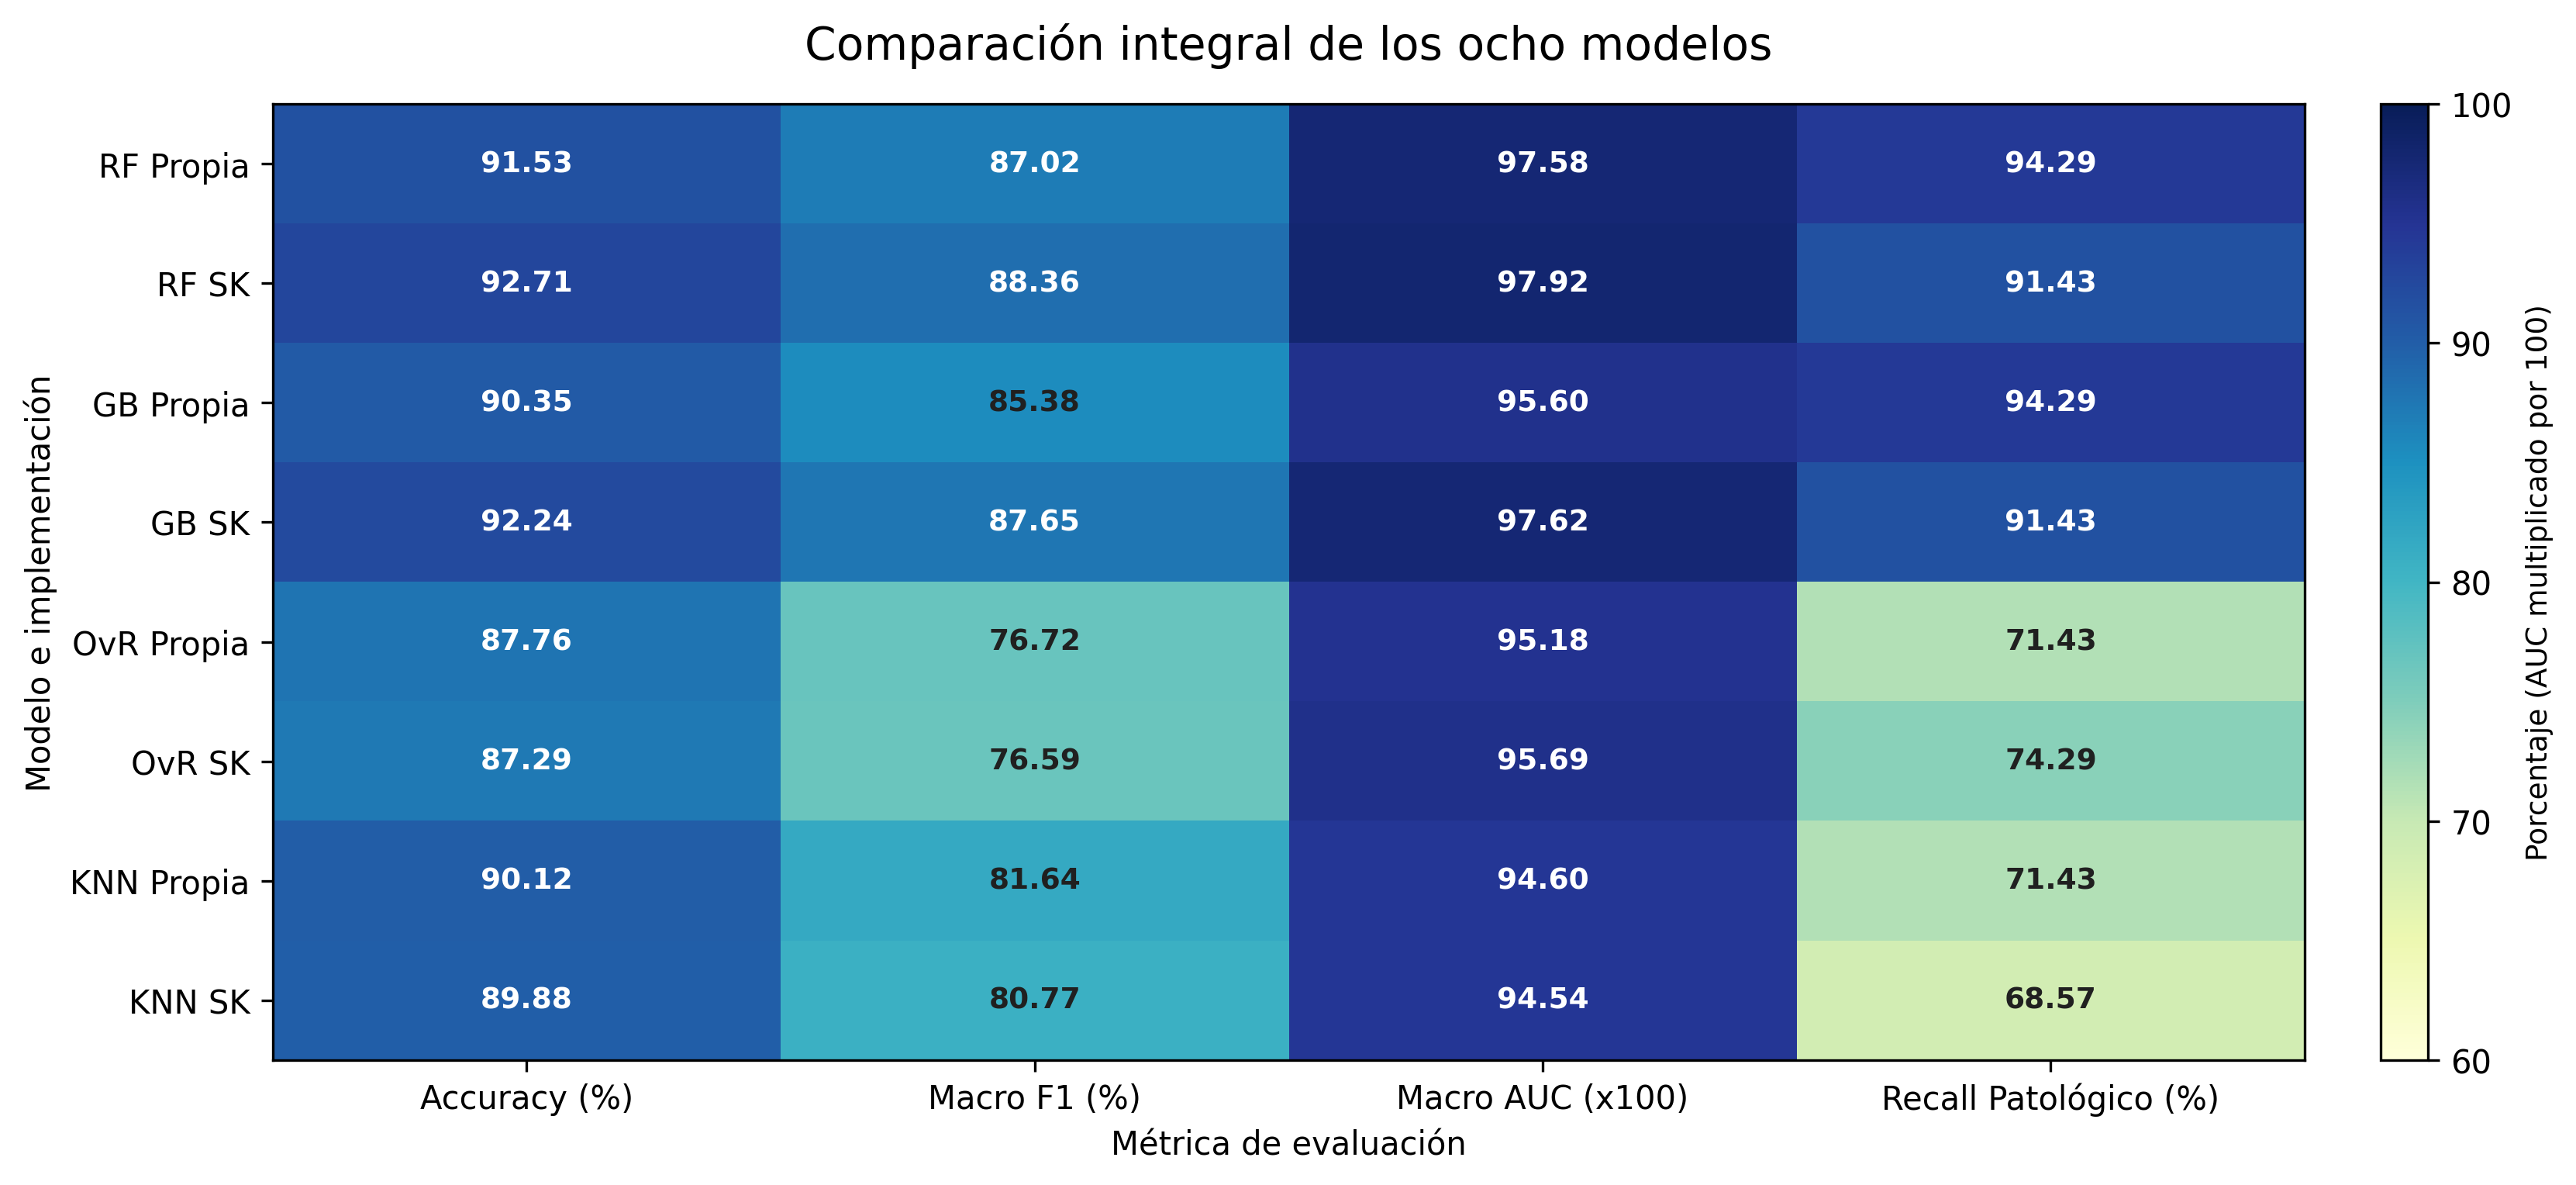
\includegraphics[width=0.88\textwidth]{comparacion_modelos_heatmap.png}
\caption{Mapa de calor de las ocho configuraciones. Macro AUC se multiplic\'o por 100 solo para la escala visual; los resultados originales no se modificaron.}
\label{fig:global}
\end{figure*}

\subsection{Desempe\~no por categor\'ia}
Las versiones propias de RF y GB alcanzaron 94.29\% de Recall patol\'ogico, equivalente a identificar 33 de los 35 registros patol\'ogicos de prueba. Sin embargo, las precisiones patol\'ogicas fueron distintas: 89.19\% para RF propio y 82.50\% para GB propio. Ambos recuperaron la misma cantidad de registros patol\'ogicos, pero GB propio gener\'o m\'as predicciones de esa clase que no correspond\'ian a casos patol\'ogicos. RF de biblioteca identific\'o 32 de los 35 casos patol\'ogicos (91.43\% de Recall), aunque obtuvo una precisi\'on mayor (96.97\%). En t\'erminos del proyecto, RF propio prioriza ligeramente la detecci\'on de m\'as casos patol\'ogicos, mientras que RF de biblioteca reduce las falsas alarmas de esa categor\'ia.

Gradient Boosting propio obtuvo el mayor Recall de la clase Sospechosa (84.75\%), lo que equivale a recuperar 50 de los 59 registros de prueba de esa categor\'ia; su precisi\'on fue 65.79\%, por lo que parte de las predicciones Sospechosas correspondieron a registros de otra clase. En contraste, OvR propio obtuvo 52.54\% de Recall Sospechoso. KNN propio identific\'o 97.28\% de los registros Normales, pero su Recall fue de 61.02\% para Sospechoso y 71.43\% para Patol\'ogico. Este contraste indica que KNN reconoce bien el patr\'on mayoritario, pero recupera en menor proporci\'on las dos clases menos frecuentes. El desbalance de NSP y la similitud entre ciertos perfiles de CTG pueden influir en este comportamiento; los resultados no permiten atribuirlo a una sola variable.

\begin{table*}[t]
\centering
\caption{Recall por clase y medidas complementarias para la clase patol\'ogica.}
\label{tab:recallclase}
\scriptsize
\begin{tabular}{llrrrrr}
\toprule
Modelo & Implementaci\'on & Recall Normal (\%) & Recall Sospechoso (\%) & Recall Patol. (\%) & Precisi\'on Patol. (\%) & F1 Patol. (\%) \\
\midrule
RF & Propia & 93.35 & 79.66 & 94.29 & 89.19 & 91.67 \\
RF & \textit{scikit-learn} & 96.37 & 72.88 & 91.43 & 96.97 & 94.12 \\
GB & Propia & 90.94 & 84.75 & 94.29 & 82.50 & 88.00 \\
GB & \textit{scikit-learn} & 94.56 & 79.66 & 91.43 & 88.89 & 90.14 \\
OvR & Propia & 95.77 & 52.54 & 71.43 & 89.29 & 79.37 \\
OvR & \textit{scikit-learn} & 94.86 & 52.54 & 74.29 & 86.67 & 80.00 \\
KNN & Propia & 97.28 & 61.02 & 71.43 & 100.00 & 83.33 \\
KNN & \textit{scikit-learn} & 97.28 & 61.02 & 68.57 & 100.00 & 81.36 \\
\bottomrule
\end{tabular}
\end{table*}

La Figura~\ref{fig:recall} complementa la tabla al comparar el Recall de las tres clases. La diferencia entre Normal y las otras categor\'ias resulta especialmente relevante para KNN y OvR. El desbalance de etiquetas y la similitud de patrones entre clases pueden influir en esa brecha; sin un an\'alisis adicional no debe atribuirse a una sola variable o mecanismo.

\begin{figure*}[t]
\centering
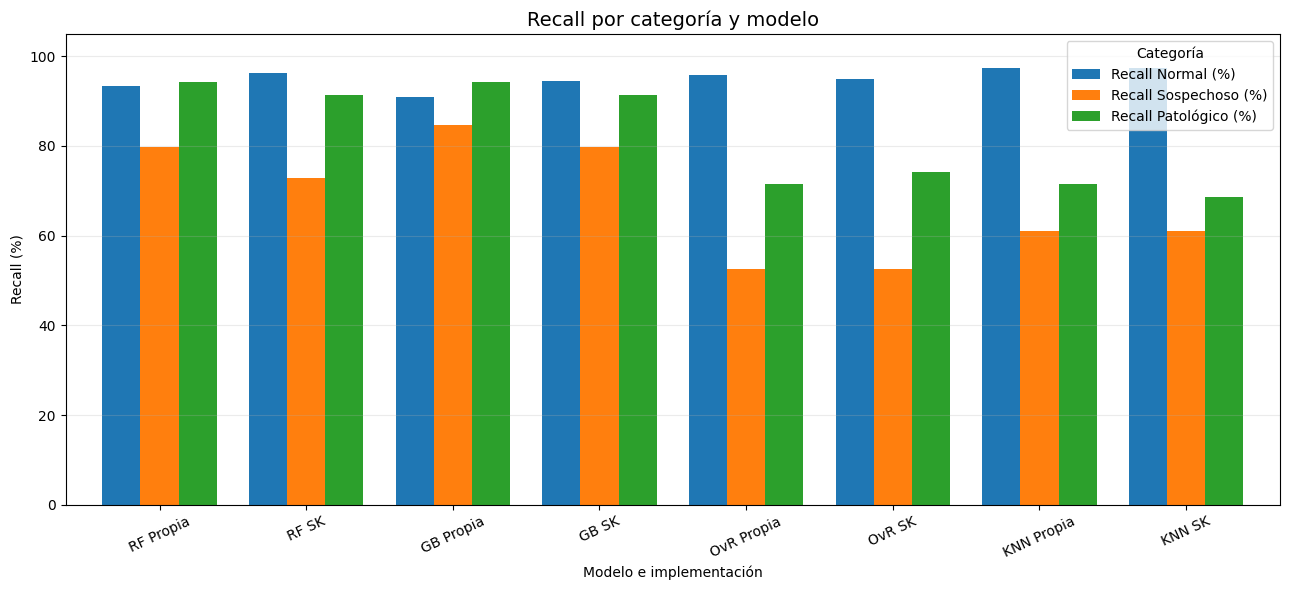
\includegraphics[width=0.89\textwidth]{recall_por_clase.png}
\caption{Recall por categor\'ia y modelo. Gr\'afica original conservada del notebook `07\_Comparacion\_Modelos.ipynb`.}
\label{fig:recall}
\end{figure*}

\subsection{Lectura integrada de los resultados en el contexto de CTG}
Las métricas por clase permiten traducir los porcentajes a registros concretos y dimensionar mejor las diferencias. En la prueba hubo 331 observaciones Normales, 59 Sospechosas y 35 Patológicas. KNN propio identificó correctamente 322 registros Normales (97.28\%), pero reconoció 36 de los 59 Sospechosos (61.02\%) y 25 de los 35 Patológicos (71.43\%). Por tanto, su buen resultado en la clase mayoritaria no se reproduce con la misma intensidad en las otras dos categorías. Este patrón es compatible con la influencia del desbalance: en una vecindad de cinco registros, los ejemplos Normales son mucho más abundantes en el conjunto de entrenamiento y pueden dominar la votación cuando los patrones se encuentran próximos.

En la clase Sospechosa, Gradient Boosting propio obtuvo el mejor Recall: identificó 50 de los 59 casos (84.75\%). RF propio y Gradient Boosting de biblioteca identificaron 47 casos cada uno (79.66\%), mientras que OvR reconoció 31 (52.54\%). La categoría Sospechosa puede reunir registros con características intermedias o compartidas con las otras clases, lo que vuelve más difícil establecer una separación consistente. Esta interpretación es una posible explicación del patrón observado, no una conclusión clínica sobre cada registro. La diferencia también muestra por qué conviene conservar las métricas por clase: un modelo puede tener un desempeño general alto y aun así dejar sin identificar una parte importante de esta categoría.

Para la clase Patológica, RF propio y Gradient Boosting propio identificaron 33 de los 35 casos de prueba (94.29\%); las versiones de biblioteca de ambos ensambles identificaron 32. OvR propio y KNN propio reconocieron 25, mientras que OvR de biblioteca reconoció 26 y KNN de biblioteca 24. Sin embargo, RF propio obtuvo 89.19\% de precisión patológica frente a 82.50\% de Gradient Boosting propio. En consecuencia, aunque ambos recuperaron el mismo número de casos, RF propio produjo una proporción mayor de predicciones patológicas correctas. RF de biblioteca alcanzó una precisión patológica de 96.97\%, con 32 casos identificados: en esta partición fue más selectivo al asignar esa etiqueta.

Estas diferencias deben interpretarse considerando el tamaño reducido de la clase Patológica en la prueba. Cada registro representa aproximadamente 2.86 puntos porcentuales de su Recall; por eso, la diferencia entre 33 y 32 casos equivale a un solo registro. En la clase Sospechosa, cada caso modifica el Recall alrededor de 1.69 puntos, mientras que en Normal el cambio por registro es de apenas 0.30 puntos. La comparación es útil para describir el comportamiento de los modelos en esta partición, pero no basta para afirmar que una variante sea estadísticamente superior a otra.

Los hallazgos del EDA también ayudan a interpretar, con cautela, las diferencias entre algoritmos. DP, ASTV y ALTV presentaron asociaciones positivas moderadas con NSP, mientras que AC mostró una asociación negativa. Los árboles pueden construir reglas por umbral y combinar varias características en diferentes ramas, por lo que su estructura permite representar relaciones no lineales entre las mediciones. Esto es compatible con el buen desempeño de los ensambles, aunque no demuestra que esas cuatro variables hayan sido las responsables: no se calculó importancia de características ni se hizo una prueba de eliminación individual.

KNN, en cambio, resume las 21 variables en una distancia conjunta. La estandarización evita que una escala domine por su magnitud, pero no elimina la información compartida entre variables correlacionadas, como Mode, Mean y Median. Esa redundancia puede influir en qué registros terminan siendo vecinos. La regresión logística OvR sirve como referencia de fronteras lineales; su menor Macro F1 y Recall en Sospechoso indican que, con la configuración utilizada, tuvo más dificultad para recuperar esa clase que los ensambles. En conjunto, los resultados sugieren que la combinación de umbrales y votaciones de los modelos de árboles se adaptó mejor a este conjunto, sin que ello permita concluir que el mismo comportamiento se mantendrá en otros datos o en un entorno clínico.

\subsection{Eficiencia computacional}
Los tiempos de la Tabla~\ref{tab:resultados} corresponden a una ejecuci\'on registrada en los notebooks. Las implementaciones de biblioteca fueron m\'as r\'apidas en los dos ensambles, con una diferencia especialmente amplia en entrenamiento. En el caso de KNN, el ajuste requiere almacenar los ejemplos, mientras que la mayor parte del c\'alculo ocurre durante la predicci\'on: por ello los tiempos de entrenamiento son muy bajos y los de inferencia comparativamente altos.

Los tiempos no constituyen un benchmark controlado. Pueden variar seg\'un hardware, carga de ejecuci\'on, versiones de bibliotecas y paralelismo disponible. En consecuencia, se presentan como evidencia descriptiva para esta ejecuci\'on y no como una propiedad universal de cada algoritmo.

\begin{figure}[!htb]
\centering
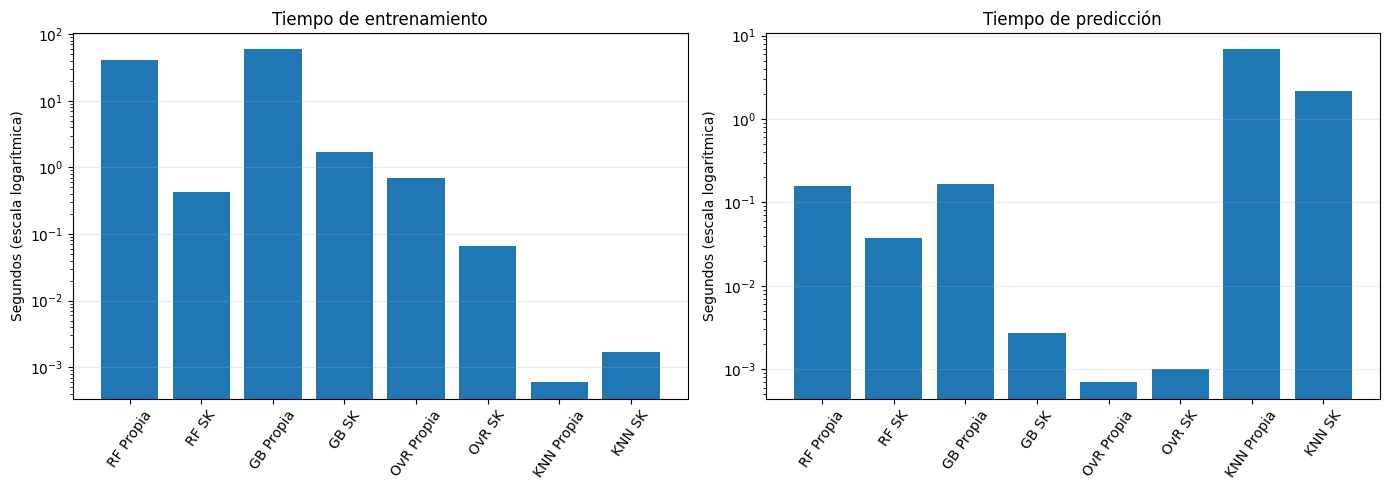
\includegraphics[width=0.96\columnwidth]{tiempos_ejecucion.png}
\caption{Tiempos de entrenamiento y predicci\'on registrados. Gr\'afica original conservada del notebook `07\_Comparacion\_Modelos.ipynb`.}
\label{fig:tiempos}
\end{figure}

\subsection{Selecci\'on e interpretaci\'on de modelos}
Si el criterio principal es el equilibrio global entre las tres clases, RF de biblioteca es la configuraci\'on mejor posicionada, al presentar la mayor Accuracy, Macro F1 y Macro AUC. Si el objetivo experimental prioriza la sensibilidad patol\'ogica, RF propio y GB propio obtienen el mayor Recall de esa clase. Entre ambos, RF propio mantiene mejor precisi\'on patol\'ogica y un F1 patol\'ogico superior, mientras que GB propio es el mejor en Recall Sospechoso. La selecci\'on final depende, por tanto, del costo relativo de falsos negativos y falsos positivos.

Las correlaciones del EDA ayudan a contextualizar, pero no explican por s\'i solas las predicciones. Los modelos recibieron las 21 caracter\'isticas y no se realiz\'o un experimento de importancia o exclusi\'on de variables para medir el efecto individual de DP, ASTV, ALTV o AC. Por ello, es razonable se\~nalar que esas variables presentan asociaciones con NSP y pueden aportar patrones aprovechables por los clasificadores, pero no afirmar que sean las responsables directas del mejor desempe\~no de Random Forest.

La comparaci\'on entre implementaciones propias y bibliotecas no es una prueba de equivalencia algor\'itmica. Las configuraciones presentan diferencias en mecanismos de balanceo, regularizaci\'on, optimizaci\'on y c\'alculo interno de los pesos. El valor del ejercicio consiste en contrastar implementaciones y observar c\'omo las decisiones algor\'itmicas afectan el desempe\~no y la eficiencia.

\subsection{Alcance de la selecci\'on seg\'un el objetivo}
La comparaci\'on permite distinguir entre un modelo con buen equilibrio general y uno que favorece la detecci\'on de una categor\'ia concreta. Si se consideran conjuntamente Accuracy, Macro F1 y Macro AUC, RF de \textit{scikit-learn} es la opci\'on experimental m\'as consistente. Adem\'as de obtener las mejores m\'etricas globales, alcanz\'o 96.97\% de precisi\'on patol\'ogica y 91.43\% de Recall en esa clase. Esto significa que sus predicciones patol\'ogicas fueron muy precisas, aunque identific\'o un caso menos que RF propio y GB propio.

Si se prioriza recuperar la mayor cantidad posible de registros patol\'ogicos, las dos implementaciones propias de ensamble identificaron 33 de 35 casos. Entre ellas, RF propio ofrece un compromiso m\'as equilibrado que GB propio en la clase Patol\'ogica, porque su precisi\'on fue mayor (89.19\% frente a 82.50\%). Por otro lado, GB propio destac\'o en la clase Sospechosa con 50 de 59 casos identificados. KNN propio ilustra por qu\'e no conviene elegir por una sola m\'etrica: obtuvo 100\% de precisi\'on patol\'ogica, pero su Recall fue 71.43\%, por lo que no identific\'o 10 de los 35 casos reales de esa clase.

En una aplicaci\'on de apoyo a la valoraci\'on fetal, tanto los casos no detectados como las alertas incorrectas tendr\'ian consecuencias distintas. Sin embargo, este proyecto no defini\'o costos cl\'inicos ni umbrales de decisi\'on con especialistas; por ello, no corresponde declarar un modelo como el m\'as seguro para uso m\'edico. La selecci\'on que se presenta es acad\'emica y depende de la m\'etrica que se desee priorizar. Para trasladar estos resultados a un contexto asistencial har\'ian falta datos independientes, validaci\'on externa y evaluaci\'on con criterios cl\'inicos.

\section{Conclusiones de la parte experimental}
En la partici\'on evaluada, RF de \textit{scikit-learn} obtuvo el mejor equilibrio global. RF propio y GB propio resultaron competitivos para la identificaci\'on de registros patol\'ogicos, ambos con 94.29\% de Recall. GB propio destac\'o adem\'as en la recuperaci\'on de registros sospechosos, aunque con menor precisi\'on en esa clase. KNN y regresi\'on log\'istica OvR aportaron referencias de m\'etodos basados, respectivamente, en vecindad y fronteras lineales.

El estudio tiene limitaciones: se utiliz\'o una sola partici\'on de entrenamiento/prueba; la clase patol\'ogica contiene 35 observaciones de prueba; y las variantes propias y de biblioteca no tienen configuraciones completamente equivalentes. Como trabajo futuro se propone aplicar validaci\'on cruzada estratificada, repetir mediciones temporales bajo condiciones controladas, explorar hiperpar\'ametros y evaluar el comportamiento con datos independientes. La clasificaci\'on reproduce la etiqueta NSP del conjunto; no establece una decisi\'on m\'edica, no sustituye la valoraci\'on profesional y no ha sido validada para uso cl\'inico.

% =====================================================================
% PARTE II: MATEMATICAS
% =====================================================================
\newpage
\section*{Parte II. Matem\'aticas Aplicadas a la Ciencia de Datos: fundamentos de los modelos utilizados}
\setcounter{section}{0}
\setcounter{subsection}{0}
Esta parte presenta los fundamentos matem\'aticos de KNN y de los \'arboles de decisi\'on con su extensi\'on Random Forest. Se priorizan las operaciones que se aplicaron en el proyecto: c\'alculo de distancias, estandarizaci\'on, reducci\'on de impureza mediante Gini, muestreo de entrenamiento y votaci\'on del ensamble. Las explicaciones se relacionan con las 21 caracter\'isticas de cardiotocograf\'ia y las tres etiquetas NSP.

\section{KNN: clasificaci\'on por vecinos cercanos}
K-Nearest Neighbors (KNN) clasifica un registro nuevo compar\'andolo con los ejemplos conocidos. En el proyecto, cada observaci\'on se representa mediante un vector de $p=21$ caracter\'isticas num\'ericas y su etiqueta pertenece a $\{1,2,3\}$: Normal, Sospechoso o Patol\'ogico. El modelo utiliza $k=5$ vecinos y distancia euclidiana.

\subsection{Distancia y estandarizaci\'on}
Para una observaci\'on nueva $\mathbf{z}$ y un registro de entrenamiento $\mathbf{x}_i$, la distancia euclidiana se calcula como:
\begin{equation}
d(\mathbf{z},\mathbf{x}_i)=\sqrt{\sum_{j=1}^{21}(z_j-x_{ij})^2}.
\end{equation}
La expresi\'on suma las diferencias entre las 21 caracter\'isticas, eleva cada diferencia al cuadrado y obtiene la ra\'iz del total. Las observaciones con menor distancia se consideran m\'as parecidas seg\'un las variables incluidas.

Antes de calcular las distancias se estandariz\'o cada variable mediante Z-score:
\begin{equation}
z_{ij}=\frac{x_{ij}-\mu_j}{\sigma_j},
\end{equation}
donde $\mu_j$ y $\sigma_j$ son la media y la desviaci\'on est\'andar de la caracter\'istica $j$. Ambas se calcularon exclusivamente con los datos de entrenamiento y se reutilizaron para transformar los datos de prueba. De esta forma, variables medidas en escalas distintas no dominan la distancia solo por tener valores num\'ericos mayores.

\subsection{Votaci\'on y predicci\'on}
Una vez calculadas las distancias, el algoritmo conserva los cinco registros m\'as cercanos. La clase predicha es la que obtiene m\'as votos:
\begin{equation}
\hat y(\mathbf{z})=\operatorname*{arg\,max}_{c\in\{1,2,3\}}
\sum_{i\in N_5(\mathbf{z})}\mathbb{I}(y_i=c),
\end{equation}
donde $N_5(\mathbf{z})$ representa los cinco vecinos y $\mathbb{I}(y_i=c)$ vale uno cuando el vecino pertenece a la clase $c$ y cero en caso contrario. La proporci\'on de votos de cada clase se obtiene dividiendo su n\'umero de votos entre cinco; el c\'odigo la utiliza como puntaje para las curvas ROC, no como una probabilidad cl\'inica calibrada.

KNN no aprende coeficientes ni construye reglas durante el ajuste. Su m\'etodo \texttt{fit} almacena los registros de entrenamiento y sus etiquetas; al predecir, calcula las distancias y ordena los resultados para encontrar los vecinos. En la implementaci\'on propia, esta b\'usqueda exhaustiva requiere aproximadamente $O(Np+N\log N)$ operaciones por consulta, donde $N$ es el n\'umero de registros de entrenamiento. Esto ayuda a explicar los tiempos registrados: el entrenamiento fue casi inmediato, pero la predicci\'on fue m\'as lenta que en los modelos basados en \'arboles.

La estandarizaci\'on iguala las escalas, pero no elimina la correlaci\'on entre variables. En nuestro EDA, estad\'isticos como Mode, Mean y Median mostraron relaciones elevadas entre s\'i. Al participar simult\'aneamente en la distancia, caracter\'isticas que describen aspectos relacionados de la se\~nal pueden dar un peso conjunto mayor a esa informaci\'on. Esto es una limitaci\'on a considerar al interpretar la vecindad, aunque no se midi\'o por separado su efecto en el resultado.

\section{\'Arboles de decisi\'on para clasificaci\'on}
Un \'arbol de decisi\'on divide los registros mediante preguntas sucesivas sobre las caracter\'isticas. Cada nodo interno eval\'ua una regla del tipo $x_j\leq\tau$: los registros que cumplen la condici\'on avanzan por una rama y los dem\'as por la otra. Las hojas contienen la clase asignada, normalmente la m\'as frecuente entre los registros que llegaron a esa regi\'on.

\subsection{Impureza Gini y selecci\'on de cortes}
Para medir qu\'e tan mezcladas est\'an las clases en un nodo $t$, se calcula la proporci\'on $p_{tc}$ de registros de cada clase. El \'indice Gini se define como:
\begin{equation}
G(t)=1-\sum_{c=1}^{3}p_{tc}^{2}.
\end{equation}
Un valor de cero indica que todos los registros del nodo pertenecen a la misma clase; valores mayores indican una mezcla m\'as equilibrada. Cuando las tres clases aparecen en la misma proporci\'on, Gini alcanza su m\'aximo de $2/3$.

Para evaluar un corte, el algoritmo compara la impureza del nodo original con el promedio ponderado de sus dos grupos resultantes:
\begin{equation}
G_{\mathrm{post}}=\frac{N_L}{N_t}G(L)+\frac{N_R}{N_t}G(R),
\qquad
\Delta G=G(t)-G_{\mathrm{post}}.
\end{equation}
$N_t$ es la cantidad de registros del nodo y $N_L$, $N_R$ son los que quedan a cada lado del corte. Se elige la caracter\'istica y el umbral que producen la mayor reducci\'on $\Delta G$; en otras palabras, el corte que deja grupos m\'as homog\'eneos en cuanto a NSP. Por ejemplo, el algoritmo podr\'ia evaluar una regla sobre DP o ASTV y conservarla si separa mejor las clases dentro del nodo. El ejemplo describe el tipo de operaci\'on, no un umbral espec\'ifico obtenido en el entrenamiento.

En el proyecto, las variables predictoras son num\'ericas y el clasificador propio utiliza divisiones binarias por umbral e \'indice Gini. El crecimiento se detiene cuando el nodo ya contiene una sola clase, no encuentra un corte v\'alido, tiene menos de dos registros para dividirse o alcanza la profundidad m\'axima de 12. Los \'arboles no requieren estandarizaci\'on: comparan valores dentro de una caracter\'istica y seleccionan umbrales, por lo que un cambio de escala no altera el orden de los registros.

\section{Random Forest: combinaci\'on de \'arboles}
Random Forest construye varios \'arboles y combina sus predicciones mediante votaci\'on. La idea es que los \'arboles no sean id\'enticos: cada uno se entrena con una muestra bootstrap (selecci\'on con reemplazo) y, en cada nodo, considera solo una parte aleatoria de las caracter\'isticas disponibles.

En nuestra implementaci\'on propia se construyeron $B=100$ \'arboles. Para cada uno se gener\'o una muestra balanceada de 1\,701 registros: 567 de cada clase, seleccionados con reemplazo. En cada divisi\'on se eligieron al azar cuatro de las 21 caracter\'isticas candidatas. Cada \'arbol produce una etiqueta $T_b(\mathbf{x})$ y el bosque asigna la clase con mayor n\'umero de votos:
\begin{equation}
\begin{aligned}
\hat y_{RF}(\mathbf{x})&=\operatorname*{arg\,max}_{c\in\{1,2,3\}}\\
&\sum_{b=1}^{100}\mathbb{I}(T_b(\mathbf{x})=c).
\end{aligned}
\end{equation}
El balanceo busca evitar que la clase Normal, mayoritaria en los datos, domine las muestras de cada \'arbol. La selecci\'on aleatoria de caracter\'isticas favorece que los \'arboles aprendan reglas diferentes; la votaci\'on combina sus resultados. La versi\'on de \textit{scikit-learn} aplica ponderaci\'on \texttt{balanced\_subsample}, que compensa el desbalance mediante pesos y no mediante la misma selecci\'on balanceada expl\'icita de la implementaci\'on propia. Por ello, las dos variantes comparten la idea de ensamble, pero no realizan exactamente el mismo procedimiento.

\subsection{Relaci\'on con los resultados del proyecto}
Random Forest de biblioteca obtuvo el mejor desempe\~no global (92.71\% de Accuracy, 88.36\% de Macro F1 y 0.9792 de Macro AUC). La versi\'on propia alcanz\'o 94.29\% de Recall patol\'ogico, equivalente a 33 de 35 casos, aunque su precisi\'on patol\'ogica fue menor que la de biblioteca. Esta diferencia refleja el equilibrio entre recuperar m\'as registros de una clase minoritaria y evitar falsas alarmas. El balanceo aplicado al bosque propio puede contribuir a que los \'arboles presten mayor atenci\'on a las clases menos frecuentes, pero no se puede atribuir el resultado a ese mecanismo de manera aislada, pues tambi\'en cambian otros detalles de implementaci\'on.

La asociaci\'on de DP, ASTV y ALTV con NSP ayuda a comprender por qu\'e caracter\'isticas relacionadas con desaceleraciones y variabilidad pueden ofrecer reglas \'utiles para separar registros. Sin embargo, como no se report\'o un an\'alisis de importancia o ablaci\'on de variables, no se afirma que sean las variables m\'as utilizadas por los \'arboles ni las responsables del rendimiento. Las correlaciones del EDA son un contexto para interpretar los datos, no una explicaci\'on causal del modelo.

En t\'erminos de complejidad, la construcci\'on del bosque repite el proceso de entrenamiento de un \'arbol $B$ veces; su costo crece con la cantidad de \'arboles y el n\'umero de cortes evaluados. Para clasificar una observaci\'on se recorren los 100 \'arboles, con una profundidad m\'axima de 12 niveles por \'arbol. Esto aumenta el costo frente a un solo \'arbol, pero permite combinar decisiones distintas y obtener una predicci\'on de conjunto.

\section{Cierre de los fundamentos matem\'aticos}
KNN y Random Forest utilizan mecanismos diferentes para interpretar las 21 mediciones de CTG. KNN compara cada registro con ejemplos cercanos y, por ello, depende de la escala y de la composici\'on de las caracter\'isticas en la distancia. Los \'arboles buscan reglas que reduzcan la mezcla de clases; Random Forest combina 100 \'arboles con muestras y subconjuntos de variables distintos. Estas operaciones explican parte de las diferencias observadas en los tiempos y en la detecci\'on de las clases NSP.

El an\'alisis se limita al conjunto utilizado y a la partici\'on de prueba descrita. Las asociaciones entre variables no prueban relaciones causales y las predicciones no constituyen diagn\'osticos. Para una evaluaci\'on posterior ser\'ia necesario validar los modelos con nuevas particiones y datos independientes.

\balance
\printbibliography[title={Referencias}]
\end{document}
